\setcounter{framenumber}{0}
%50

\begin{frame}
  \titlepage
\end{frame}

\begin{frame}{Learning Goals}
By the end of this lecture, students should be able to:
\begin{itemize}
    \item define expectation for discrete random variables;
    \item compute expectations from PMFs;
    \item use linearity of expectation;
    \item use indicator random variables and the fundamental bridge;
    \item define and compute variance and standard deviation;
    \item understand the Poisson approximation to the Binomial;
    \item know the expectations of the main discrete distributions.
\end{itemize}
\end{frame}

\lecturepart{Definition of Expectation}

\begin{frame}{Why Expectation?}
A distribution gives detailed information about a random variable:
\[
\Prob(X=x), \qquad \Prob(X\leq x), \qquad \Prob(a\leq X\leq b).
\]

\vspace{0.25cm}

But sometimes we want a single number summarizing the ``average'' value of $X$.

\vspace{0.25cm}

\begin{keybox}{Main idea}
The expected value of a random variable is its probability-weighted average.
\end{keybox}
\end{frame}

\begin{frame}{Idea: (Weighted) Averages}
For ordinary numbers
\[
x_1,x_2,\dots,x_n,
\]
the usual average is
\begin{equation} \label{avg}
    \bar x = \frac{1}{n} \sum_{i=1}^n x_j 
\end{equation}

More generally, if
\[
p_1,\dots,p_n\geq0,
\qquad
\sum_{j=1}^n p_j=1,
\]
then the weighted average is
\[
\sum_{j=1}^n x_jp_j.
\]

Note that equation \eqref{avg} uses equal weights $p_j= \frac{1}{n}, \ \forall j=1,\dots, n$, so it is a special case.
 


\end{frame}

\begin{frame}{Definition: Expected Value}
\begin{keybox}{Definition (Expected value of a discrete r.v.)}
Let $X$ be a discrete random variable with possible values
\[
x_1,x_2,\dots.
\]

The expected value of $X$ is
\[
\boxed{
\mathbb{E}(X)=\sum_j x_j\Prob(X=x_j).
}
\]
\end{keybox}

Equivalently,
\[
\mathbb{E}(X)=\sum_{x_j} x_j\,p_X(x_j),
\]
where
\[
p_X(x)=\Prob(X=x).
\]

\begin{keybox}{Interpretation}
Expectation is the center of mass of the PMF (next slide).
\end{keybox}
\end{frame}


\begin{frame}{Expectation as a Center of Mass (Proof is Optional)}

Suppose a discrete random variable \(X\) takes values
\[
x_1,x_2,\dots
\]
with probabilities
\[
p_1,p_2,\dots
\]

Think of the PMF as placing masses \(p_i\) at locations \(x_i\) on the number line.

The \textbf{center of mass} (balance point) is a point \(c\) such that
\[
\sum_i (x_i-c)p_i = 0.
\]

This means:
\begin{itemize}
    \item points to the right of \(c\) pull one way,
    \item points to the left of \(c\) pull the other way,
    \item and the system balances perfectly at \(c\).
\end{itemize}
Expanding the equation:
\[
\sum_i x_i p_i - c\sum_i p_i = 0.
\]

Since
\[
\sum_i p_i = 1,
\]
we obtain
\[
c = \sum_i x_i p_i = \mathbb{E}[X].
\]

\end{frame}











\begin{frame}{Example: One Fair Die}
Let
\[
X=\text{result of one fair die roll}.
\]

Then
\[
\Prob(X=k)=\frac16,
\qquad k=1,2,\dots,6.
\]

Thus
\[
\mathbb{E}(X)
=
\sum_{k=1}^6 k\Prob(X=k)
=\sum_{k=1}^6 k\times \frac{1}{6}= 
\frac{1+2+3+4+5+6}{6}.
\]

So
\[
{\mathbb{E}(X)=3.5.}
\]

\begin{keybox}{Important}
The expectation does not have to be a possible value of $X$.
\end{keybox}
\end{frame}

\begin{frame}{Example: Bernoulli}
Let
\[
X\sim \operatorname{Bern}(p).
\]

Then
\[
\Prob(X=1)=p,
\qquad
\Prob(X=0)=1-p.
\]

Therefore
\[
\mathbb{E}(X)
=
1\cdot p+0\cdot(1-p)
=
p.
\]

So
\[
{\mathbb{E}(X)=p.}
\]
\end{frame}




\begin{frame}{Example: Discrete Uniform}
Let
\[
X\sim \operatorname{DUnif}(\{a,a+1,\dots,b\}).
\]

All values are equally likely.

There are
\[
b-a+1
\]
possible values.

Thus
\[
\mathbb{E}(X)
=
\frac{a+(a+1)+\cdots+b}{b-a+1}.
\]

The average of equally spaced endpoints is the midpoint:

\[
\boxed{
\mathbb{E}(X)=\frac{a+b}{2}.
}
\]
\end{frame}



% -------------------------------------------------------


% -------------------------------------------------------

\begin{frame}{Example: Geometric Distribution}
Let
\[
X\sim \operatorname{Geom}(p).
\]

Recall:
\[
\Prob(X=k)
=
(1-p)^{k-1}p,
\qquad
k=1,2,\dots
\]

Then
\[
\mathbb{E}(X)
=
\sum_{k=1}^{\infty}
k(1-p)^{k-1}p.
\]

Using the geometric-series identity,
\[
\sum_{k=1}^\infty kr^{k-1}
=
\frac1{(1-r)^2},
\qquad |r|<1,
\]
with $r=1-p$, we obtain

\[
{
\mathbb{E}(X)=\frac1p.
}
\]
\end{frame}

% -------------------------------------------------------

\begin{frame}{Example: Negative Binomial Distribution}
Let
\[
X\sim \operatorname{NegBin}(r,p),
\]
where $X$ counts the number of trials needed to obtain $r$ successes.

Write
\[
X=X_1+\cdots+X_r,
\]
where each
\[
X_i\sim \operatorname{Geom}(p).
\]

Therefore,
\[
\mathbb{E}(X)
=
r\cdot \frac1p.
\]

Hence
\[
{
\mathbb{E}(X)=\frac{r}{p}.
}
\]
\end{frame}

% -------------------------------------------------------



% -------------------------------------------------------

\begin{frame}{Example: Poisson Distribution}
Let
\[
X\sim \operatorname{Pois}(\lambda).
\]

Recall:
\[
\Prob(X=k)
=
e^{-\lambda}
\frac{\lambda^k}{k!},
\qquad
k=0,1,2,\dots
\]

Then
\[
\mathbb{E}(X)
=
\sum_{k=0}^{\infty}
k
e^{-\lambda}
\frac{\lambda^k}{k!}.
\]

Rearranging,
\[
=
\lambda e^{-\lambda}
\sum_{k=1}^{\infty}
\frac{\lambda^{k-1}}{(k-1)!}.
\]

Since
\[
\sum_{j=0}^\infty
\frac{\lambda^j}{j!}
=
e^\lambda,
\]
we obtain

\[
{
\mathbb{E}(X)=\lambda.
}
\]
\end{frame}











\begin{frame}{Expectation Depends Only on the Distribution}
\begin{keybox}{Proposition}
If $X$ and $Y$ have the same distribution, then
\[
\mathbb{E}(X)=\mathbb{E}(Y),
\]
provided the expectations exist.
\end{keybox}


Reason: the formula
\[
\mathbb{E}(X)=\sum_x x\Prob(X=x)
\]
depends only on the PMF of $X$.

\vspace{0.25cm}

\begin{livebox}{Warning}
The converse is false: two random variables can have the same expectation but different distributions.
\end{livebox}
\end{frame}


\lecturepart{Linearity of Expectation}

\begin{frame}{Linearity of Expectation}
\begin{keybox}{Theorem}
For random variables $X,Y$ and constant $c$,
\[
\boxed{
\mathbb{E}(X+Y)=\mathbb{E}(X)+\mathbb{E}(Y).
}
\]

Also,
\[
\boxed{
\mathbb{E}(cX)=c\mathbb{E}(X).
}
\]
\end{keybox}

\vspace{0.25cm}

More generally,
\[
\mathbb{E}\left(\sum_{j=1}^n c_jX_j\right)
=
\sum_{j=1}^n c_j\mathbb{E}(X_j).
\]
\end{frame}



\begin{frame}{Application of Linearity in finding the Expectation of Bin(n,p)}
Let
\[
X\sim \operatorname{Bin}(n,p).
\]

Think of $X$ as the number of successes in $n$ Bernoulli trials.

Write
\[
X=I_1+\cdots+I_n,
\]
where
\[
I_j=
\begin{cases}
1,&\text{success on trial }j,\\
0,&\text{otherwise}.
\end{cases}
\]

Each
\[
I_j\sim \operatorname{Bern}(p),
\]
so
\[
\mathbb{E}(I_j)=p.
\]

Therefore, by linearity of expectation,
\[
\mathbb{E}(X)
=
\mathbb{E}[I_1 + \dots + I_n]
=
\mathbb{E}[I_1] + \dots + \mathbb{E}[I_n]
=
\underbrace{p+\dots+p}_{n\text{ times}}
=
np.
\]

Note that we did not even use the PMF of $Ber(n,p)$ to find its expectation using the main formula, which made it much easier computationally.
\end{frame}

\begin{frame}{Example: Hypergeometric Expectation}
Let
\[
X\sim \operatorname{HGeom}(w,b,n),
\]
where $X$ is the number of white balls in a sample of size $n$ drawn without replacement.

Write
\[
X=I_1+\cdots+I_n,
\]
where $I_j=1$ if the $j$th draw is white.

For each $j$,
\[
\Prob(I_j=1)=\frac{w}{w+b}.
\]

So
\[
\mathbb{E}(I_j)=\frac{w}{w+b}.
\]

By linearity,
\[
\boxed{
\mathbb{E}(X)=n\frac{w}{w+b}.
}
\]

\begin{livebox}{Key point}
The draws are dependent, but linearity still works.
\end{livebox}
\end{frame}

\begin{frame}{Monotonicity of Expectation}
\begin{keybox}{Theorem}
If
\[
X\geq Y
\]
with probability $1$, then
\[
\mathbb{E}(X)\geq \mathbb{E}(Y).
\]
\end{keybox}

\vspace{0.25cm}

Sketch of proof:
\[
X-Y\geq 0.
\]

Therefore,
\[
\mathbb{E}(X-Y)\geq0.
\]

By linearity,
\[
\mathbb{E}(X)-\mathbb{E}(Y)\geq0.
\]

For a concise proof, we need more technical tools that are not covered in this course.
\end{frame}














\lecturepart{Indicator Random Variables and the Fundamental Bridge}

\begin{frame}{Indicator Random Variables}
For an event $A$, define
\[
I_A=
\begin{cases}
1,&\text{if }A\text{ occurs},\\
0,&\text{if }A\text{ does not occur}.
\end{cases}
\]

\vspace{0.25cm}

Then
\[
I_A\sim \operatorname{Bern}(\Prob(A)).
\]

\vspace{0.25cm}

\begin{keybox}{Interpretation}
Indicators convert events into random variables.
\end{keybox}
\end{frame}

\begin{frame}{Basic Indicator Properties}
For events $A$ and $B$:

\[
I_{A^c}=1-I_A.
\]

\[
I_{A\cap B}=I_AI_B.
\]

\[
I_{A\cup B}=I_A+I_B-I_AI_B.
\]

\vspace{0.25cm}

\begin{keybox}{Reason}
Indicators behave like yes/no algebra:
\[
1=\text{yes},
\qquad
0=\text{no}.
\]
\end{keybox}
\end{frame}

\begin{frame}{The Fundamental Bridge}
\begin{keybox}{Fundamental Bridge}
For any event $A\subseteq \Sample$,
\[
\boxed{
\mathbb{E}(I_A)=\Prob(A).
}
\]
\end{keybox}

\vspace{0.25cm}

Proof:
\[
I_A\sim \operatorname{Bern}(\Prob(A)).
\]

Since the expectation of a Bernoulli random variable is its success probability,
\[
\mathbb{E}(I_A)=\Prob(A).
\]

\vspace{0.25cm}

\begin{keybox}{Meaning}
Probability questions can often be turned into expectation questions, and vice versa.
\end{keybox}
\end{frame}


\begin{frame}{Example: Matching Problem}
A deck has cards labeled
\[
1,2,\dots,n.
\]

After shuffling, a match occurs if card $j$ is in position $j$.

Let
\[
X=\text{number of matches}.
\]

Define
\[
I_j=
\begin{cases}
1,&\text{card }j\text{ is in position }j,\\
0,&\text{otherwise}.
\end{cases}
\]

Then
\[
X=I_1+\cdots+I_n.
\]

Since
\[
\Prob(I_j=1)=\frac1n,
\]
we get
\[
\mathbb{E}(X)=n\cdot\frac1n=1.
\]

\[
\boxed{\mathbb{E}(X)=1.}
\]
\end{frame}

\begin{frame}{Example: Birthday Matches}
Suppose there are $n$ people.

Let
\[
X=\text{number of pairs of people with the same birthday}.
\]

There are
\[
\binom{n}{2}
\]
pairs.

For each pair $(i,j)$, define
\[
I_{ij}=
\begin{cases}
1,&\text{people }i,j\text{ have the same birthday},\\
0,&\text{otherwise}.
\end{cases}
\]

Then
\[
X=\sum_{i<j} I_{ij}.
\]

Since
\[
\mathbb{E}(I_{ij})=\Prob(I_{ij}=1)=\frac1{365},
\]
we have
\[
{
\mathbb{E}(X)=\binom{n}{2}\frac1{365}.
}
\]
\end{frame}

\lecturepart{Variance}

\begin{frame}{Why Variance?}
Expectation measures the center of a distribution.

But two distributions can have the same expectation and very different spread.

We need a numerical measure of variability.

Variance measures the average squared distance from the mean.


\begin{center}
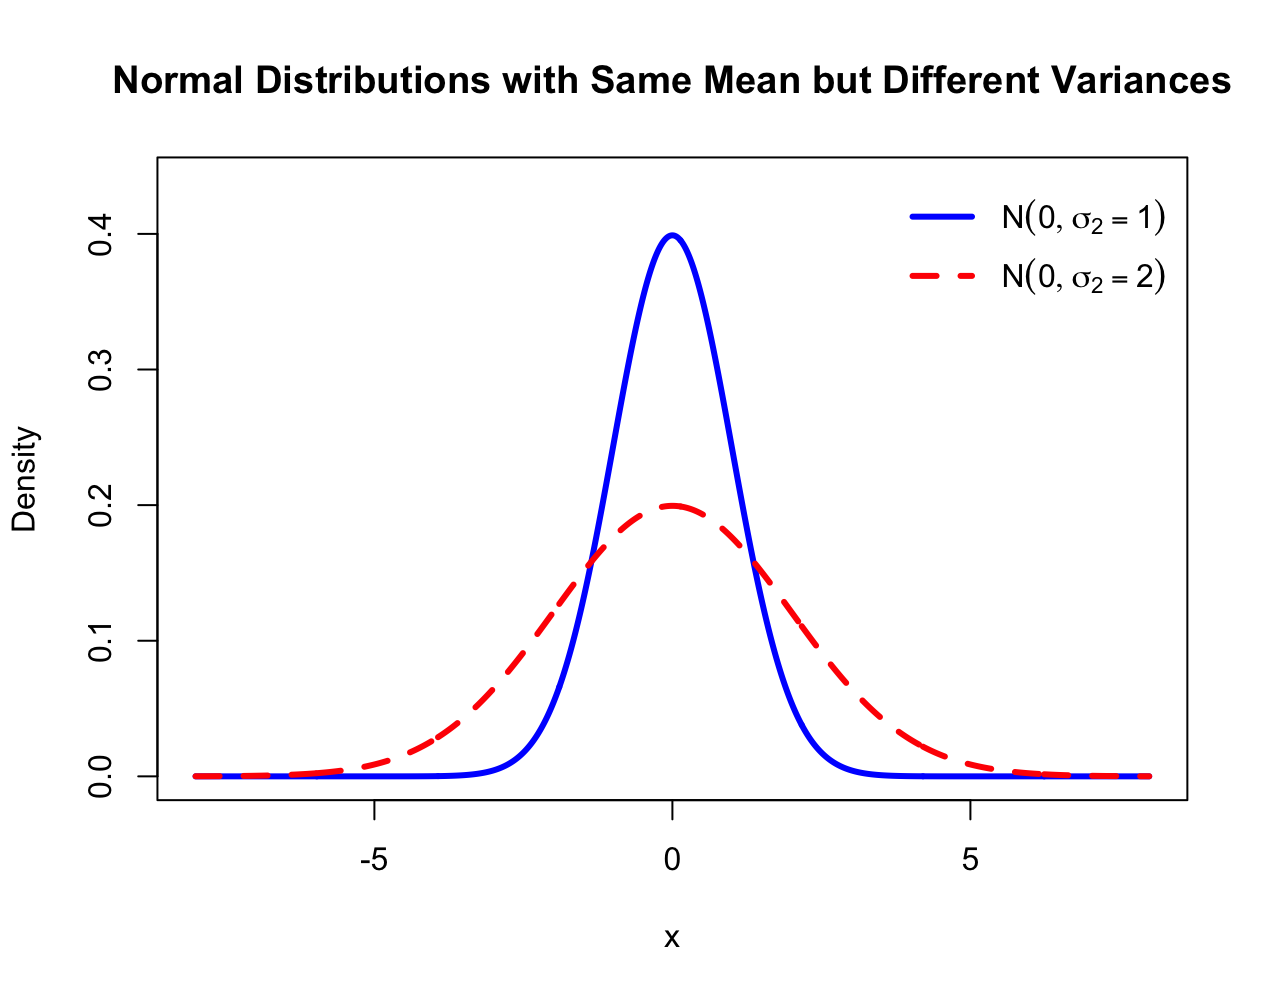
\includegraphics[width=0.5\textwidth]{assets/figures/var.png}
\end{center}
\end{frame}

\begin{frame}{Definition: Variance and Standard Deviation}
\begin{keybox}{Definition}
The variance of $X$ is
\[
\boxed{
\operatorname{Var}(X)
=
\mathbb{E}\left[(X-\mathbb{E}X)^2\right].
}
\]
Variance is a measure of dispersion (from the mean). It is a measure of how far a set of numbers are spread out from their mean, on average.
\end{keybox}

\vspace{0.25cm}

The standard deviation is
\[
\boxed{
\operatorname{SD}(X)=\sqrt{\operatorname{Var}(X)}.
}
\]

\vspace{0.25cm}

Variance has squared units; standard deviation returns to the original units.
\end{frame}


\begin{frame}{Motivation behind the formula \( \mathbb{E}[X-\mathbb{E}[X]]^2\)?}

Consider the function
\[
g(c)=\mathbb{E}\big[(X-c)^2\big].
\]

The quantity \(g(c)\) measures the average squared distance
between \(X\) and the constant \(c\).


We claim that \(g(c)\) is minimized when
\[
c=\mathbb{E}[X].
\]


Expand the square:
\[
\begin{aligned}
g(c)
&=
\mathbb{E}\left[(X-\mathbb{E}[X]+\mathbb{E}[X]-c)^2\right]
\\
&=
\mathbb{E}\left[(X-\mathbb{E}[X])^2\right]
+
2(\mathbb{E}[X]-c)\,
\mathbb{E}[X-\mathbb{E}[X]]
\\
&\qquad
+
(\mathbb{E}[X]-c)^2.
\end{aligned}
\]

Since $\mathbb{E}[X-\mathbb{E}[X]]=0,
$, we obtain $g(c)
=
\operatorname{Var}(X)
+
(\mathbb{E}[X]-c)^2.$

Because
\[
(\mathbb{E}[X]-c)^2\geq0,
\]
the minimum occurs when
\[
c=\mathbb{E}[X].
\]



Thus, the expectation is the \emph{best constant predictor}
of \(X\) in mean squared error.
\end{frame}








\begin{frame}{Alternative Formula for Variance}
\begin{keybox}{Variance Formula}
\[
\boxed{
\operatorname{Var}(X)
=
\mathbb{E}(X^2)-(\mathbb{E}X)^2.
}
\]
\end{keybox}

\vspace{0.25cm}

Proof :
Let
\[
\mu=\mathbb{E}X.
\]

Then
\[
\operatorname{Var}(X)
=
\mathbb{E}\left[(X-\mu)^2\right].
\]

Expanding:
\[
\mathbb{E}(X^2-2\mu X+\mu^2)
=
\mathbb{E}(X^2)-2\mu\mathbb{E}(X)+\mu^2.
\]

Since $\mu=\mathbb{E}X$,
\[
\operatorname{Var}(X)=\mathbb{E}(X^2)-\mu^2.
\]
\end{frame}

\begin{frame}{Properties of Variance}
Shifting does not change spread. Scaling by $b$ scales squared distances by $b^2$.
\[
\boxed{
\operatorname{Var}(X+a)=\operatorname{Var}(X) \quad and \quad \operatorname{Var}(bX)=b^2\operatorname{Var}(X).
}
\]
\begin{keybox}{Warning}
Unlike Expectation, Variance is not linear, i.e., in general,
\[
\operatorname{Var}(X+Y)
\neq
\operatorname{Var}(X)+\operatorname{Var}(Y).
\]
 In fact, 
\begin{equation}
    Var(X+Y) = Var(X) + Var(Y) + 2Cov(X,Y)
\end{equation}
and for $n>1$ random variables,
\begin{equation}
    Var(\sum_{i=1}^nX_i) = \sum_{i=1}^n Var(X_i) + \sum_{i\neq j}Cov(X_i,X_j)
\end{equation}
We will study this in further depth in Chapter 7 (Joint Distributions).
\end{keybox}
\end{frame}



\begin{frame}{Variance of a Binomial Random Variable}
Let
\[
X\sim \operatorname{Bin}(n,p).
\]

Write
\[
X=I_1+\cdots+I_n,
\]
where the $I_j$ are independent Bernoulli$(p)$ random variables.

Each has variance
\[
\operatorname{Var}(I_j)=p(1-p).
\]

Since the indicators are independent (*),
\[
\operatorname{Var}(X)
=
\sum_{j=1}^n \operatorname{Var}(I_j).
\]

Therefore
\[
{
\operatorname{Var}(X)=np(1-p).
}
\]

(*): Note that we previously proved that the expected value of a sum of random variables
is equal to the sum of their expected values. However, this property does
\emph{not} generally hold for variance. In general, the variance of a sum is
\emph{not} equal to the sum of the variances. Variances add only in the special case where the random variables have zero
covariance, that is, when they are uncorrelated. In particular, independence implies zero covariance, so variances of independent random variables do add. We will study covariance, correlation, and independence in more detail later. For a direct derivation of the variance of the Binomial distribution using its
PMF, \href{https://proofwiki.org/wiki/Variance_of_Binomial_Distribution}{click here}.

\end{frame}



\begin{frame}{A Useful Variance Formula (exercise)}
Show that for any random variable $X$,

\[
\operatorname{Var}(X)=\mathbb{E}[X(X-1)]+\mathbb{E}[X]-(\mathbb{E}[X])^2.
\]

\end{frame}

% --------------------------------------------------------

\begin{frame}{Discrete Uniform Variance}

Let
\[
X\sim \text{DUnif}\{1,2,\dots,n\}.
\]

Then
\[
\mathbb{E}[X]=\frac{n+1}{2}.
\]

Also,

\[
\mathbb{E}[X^2]
=
\frac1n\sum_{k=1}^n k^2
=
\frac1n\cdot \frac{n(n+1)(2n+1)}{6}
=
\frac{(n+1)(2n+1)}{6}.
\]

Therefore,

\[
\operatorname{Var}(X)
=
\mathbb{E}[X^2]-(\mathbb{E}[X])^2.
\]

\[
{
\operatorname{Var}(X)=\frac{n^2-1}{12}.
}
\]

\end{frame}

% --------------------------------------------------------

\begin{frame}{Poisson Variance}

Let
\[
X\sim \text{Pois}(\lambda).
\]

Then

\[
\Prob(X=k)=e^{-\lambda}\frac{\lambda^k}{k!},
\qquad k=0,1,2,\dots
\]

We use

\[
\mathbb{E}[X(X-1)]
=
\sum_{k=0}^\infty k(k-1)e^{-\lambda}\frac{\lambda^k}{k!}.
\]

For $k\geq 2$,

\[
k(k-1)\frac{\lambda^k}{k!}
=
\frac{\lambda^k}{(k-2)!}.
\]

Thus,

\[
\mathbb{E}[X(X-1)]
=
\lambda^2 e^{-\lambda}
\sum_{j=0}^\infty \frac{\lambda^j}{j!}
=
\lambda^2.
\]

\end{frame}

% --------------------------------------------------------

\begin{frame}{Poisson Variance Continued}

Since

\[
\mathbb{E}[X]=\lambda,
\]

we get

\[
\operatorname{Var}(X)
=
\mathbb{E}[X(X-1)]+\mathbb{E}[X]-(\mathbb{E}[X])^2.
\]

Therefore,

\[
\operatorname{Var}(X)
=
\lambda^2+\lambda-\lambda^2.
\]

\[
{
\operatorname{Var}(X)=\lambda.
}
\]

\vspace{0.25cm}

So for a Poisson random variable,

\[
{
\mathbb{E}[X]=\operatorname{Var}(X)=\lambda.
}
\]

\end{frame}

% --------------------------------------------------------

\begin{frame}{Geometric Variance}

Let
\[
X\sim \text{Geom}(p),
\]
where
\[
X=\text{number of trials until the first success}.
\]

Thus,

\[
\Prob(X=k)=(1-p)^{k-1}p,
\qquad k=1,2,3,\dots
\]

Let $q=1-p.$ Then

\[
\mathbb{E}[X]=\frac1p.
\]

A standard power series identity gives

\[
\sum_{k=1}^\infty k^2 q^{k-1}
=
\frac{1+q}{(1-q)^3}.
\]

Therefore,

\[
\mathbb{E}[X^2]
=
p\sum_{k=1}^\infty k^2q^{k-1}
=
p\cdot \frac{1+q}{(1-q)^3}.
\]

\end{frame}

% --------------------------------------------------------

\begin{frame}{Geometric Variance Continued}

Since

\[
1-q=p,
\]

we have

\[
\mathbb{E}[X^2]
=
p\cdot \frac{1+q}{p^3}
=
\frac{1+q}{p^2}.
\]

Thus,

\[
\operatorname{Var}(X)
=
\mathbb{E}[X^2]-(\mathbb{E}[X])^2.
\]

So

\[
\operatorname{Var}(X)
=
\frac{1+q}{p^2}
-
\frac{1}{p^2}
=
\frac{q}{p^2}.
\]

Since $q=1-p$,

\[
{
\operatorname{Var}(X)=\frac{1-p}{p^2}.
}
\]

\end{frame}

% --------------------------------------------------------

\begin{frame}{Negative Binomial Variance}

Let
\[
X\sim \text{NegBin}(r,p),
\]
where
\[
X=\text{number of trials needed to obtain } r \text{ successes}.
\]

A Negative Binomial random variable can be written as a sum of $r$ independent Geometric random variables:

\[
X=G_1+G_2+\cdots+G_r,
\]

where each

\[
G_i\sim \text{Geom}(p).
\]

Each $G_i$ is the waiting time for one additional success.

\end{frame}

% --------------------------------------------------------

\begin{frame}{Negative Binomial Variance Continued}

Since

\[
X=G_1+\cdots+G_r
\]

and the $G_i$ are independent,

\[
\operatorname{Var}(X)
=
\operatorname{Var}(G_1)+\cdots+\operatorname{Var}(G_r).
\]

From the Geometric variance formula,

\[
\operatorname{Var}(G_i)=\frac{1-p}{p^2}.
\]

Therefore,

\[
\operatorname{Var}(X)
=
r\cdot \frac{1-p}{p^2}.
\]

\[
{
\operatorname{Var}(X)=\frac{r(1-p)}{p^2}.
}
\]

\end{frame}

% --------------------------------------------------------

\begin{frame}{Hypergeometric Variance}

Let
\[
X\sim \text{HGeom}(w,b,n),
\]
where an urn has $w$ white balls and $b$ black balls.

Let

\[
N=w+b.
\]

We draw $n$ balls without replacement, and

\[
X=\text{number of white balls selected}.
\]

Write

\[
X=I_1+I_2+\cdots+I_n,
\]

where

\[
I_j=
\begin{cases}
1, & \text{if draw } j \text{ is white},\\
0, & \text{otherwise}.
\end{cases}
\]

\end{frame}

% --------------------------------------------------------

\begin{frame}{Hypergeometric Variance Continued}

Each indicator satisfies

\[
\mathbb{E}[I_j]=\frac{w}{N}.
\]
This feels straightforward (naive probability), but I think we should not be that comfortable with it because the draws are dependent (without replacement)! So the $j^{th}$ draw depends on the $(j-1)^{th}$ draw. But you can prove (by conditioning, on the first draw) that the second draw has expected value $w/N$, and so on for the next draw, by conditioning on the previous draws.

So

\[
\mathbb{E}[X]=\sum_{i=1}^n  \mathbb{E} [I_j] = \sum_{i=1}^n w/N=    n\frac{w}{N}.
\]

Also,

\[
\operatorname{Var}(I_j)=\frac{w}{N}\left(1-\frac{w}{N}\right).
\]

Because sampling is without replacement, the indicators are not independent.

For $i\neq j$,

\[
\Cov(I_i,I_j)
=
-\frac{w}{N}\frac{b}{N}\frac{1}{N-1}.
\]

\end{frame}

% --------------------------------------------------------

\begin{frame}{Hypergeometric Variance Formula}

Using

\[
\operatorname{Var}(X)
=
\sum_{j=1}^n \operatorname{Var}(I_j)
+
2\sum_{i<j}\Cov(I_i,I_j),
\]

we get

\[
\operatorname{Var}(X)
=
n\frac{w}{N}\frac{b}{N}
-
n(n-1)\frac{w}{N}\frac{b}{N}\frac{1}{N-1}.
\]

Factor:

\[
\operatorname{Var}(X)
=
n\frac{w}{N}\frac{b}{N}
\left(
1-\frac{n-1}{N-1}
\right).
\]

Therefore,

\[
{
\operatorname{Var}(X)
=
n\frac{w}{N}\frac{b}{N}
\frac{N-n}{N-1}.
}
\]

\end{frame}






\begin{frame}{Nonnegativity of Variance}
\begin{keybox}{Proposition} For any r.v. $X$,
\[
\operatorname{Var}(X)\geq0.
\]
\end{keybox}

\vspace{0.25cm}

Reason:
\[
(X-\mathbb{E}X)^2\geq0.
\]

Thus its expectation is nonnegative.

Later, we will learn the Jensen's Inequality, which implies this Proposition as a special case.

Also,
\[
\operatorname{Var}(X)=0
\]
if and only if $X$ is constant with probability $1$.
\end{frame}

\lecturepart{Poisson Approximation to Binomial}

\begin{frame}{Poisson Approximation to Binomial}

When
\[
X\sim \operatorname{Bin}(n,p).
\]

AND

\begin{itemize}
    \item $n$ is large;
    
    \item $p$ is small;
    
    \item  $\lambda=np$ is moderate,
\end{itemize}
Then,

\[
\boxed{
X\approx \operatorname{Pois}(\lambda).
}
\]

That is,

\[
\Prob(X=k) = \binom{n}{k}p^k(1-p)^{n-k}
\approx
e^{-\lambda}\frac{\lambda^k}{k!}.
\]

\vspace{0.25cm}


\end{frame}




\begin{frame}{Why the Poisson Approximation Works}

Assume $X\sim \operatorname{Bin}(n,p)$ with $p=\lambda/n$, where $\lambda>0$ is fixed.  For each fixed $k=0,1,2,\dots$, we have
\[
\begin{aligned}
\mathbb{P}_{Binom(n,p)}(X=k)
&=
\binom{n}{k}
\left(\frac{\lambda}{n}\right)^k
\left(1-\frac{\lambda}{n}\right)^{n-k} = \frac{n!}{k!(n-k)!}\frac{\lambda^k}{n^k}(1-\frac{\lambda}{n})^n(1-\frac{\lambda}{n})^{-k}
\\[0.2cm]
&=
\underbrace{
\left[
\left(1\right)
\left(1-\frac1n\right)
\left(1-\frac2n\right)
\cdots
\left(1-\frac{k-1}{n}\right)
\right]
}_{\longrightarrow\;1}
\;
\underbrace{
\frac{\lambda^k}{k!}
}_{\text{stays fixed}}
\;
\underbrace{
\left(1-\frac{\lambda}{n}\right)^n
}_{\longrightarrow\;e^{-\lambda}}
\;
\underbrace{
\left(1-\frac{\lambda}{n}\right)^{-k}
}_{\longrightarrow\;1}\\
&\longrightarrow
1\cdot \frac{\lambda^k}{k!}\cdot e^{-\lambda}\cdot 1
=
{
e^{-\lambda}\frac{\lambda^k}{k!}
} = \mathbb{P}_{X\sim Poisson(\lambda)}(X=k)
\end{aligned}
\]

Thus,

\[
{
\Prob_{X\sim Bin(n,p)}(X=k)
\xrightarrow[]{n\to \infty}
e^{-\lambda}\frac{\lambda^k}{k!}.
}
\]

This phenomenon is formally known as convergence in distribution (or weak convergence) in Probability theory. We will see more with Central Limit Theorem (CLT) and Law of Large Numbers (LLN) in Chapter 10B (Limit Theorems).


\end{frame}

















% -------------------------------------------------------



\begin{frame}{Visualization of Poisson Approximation to the Binomial}

\begin{center}

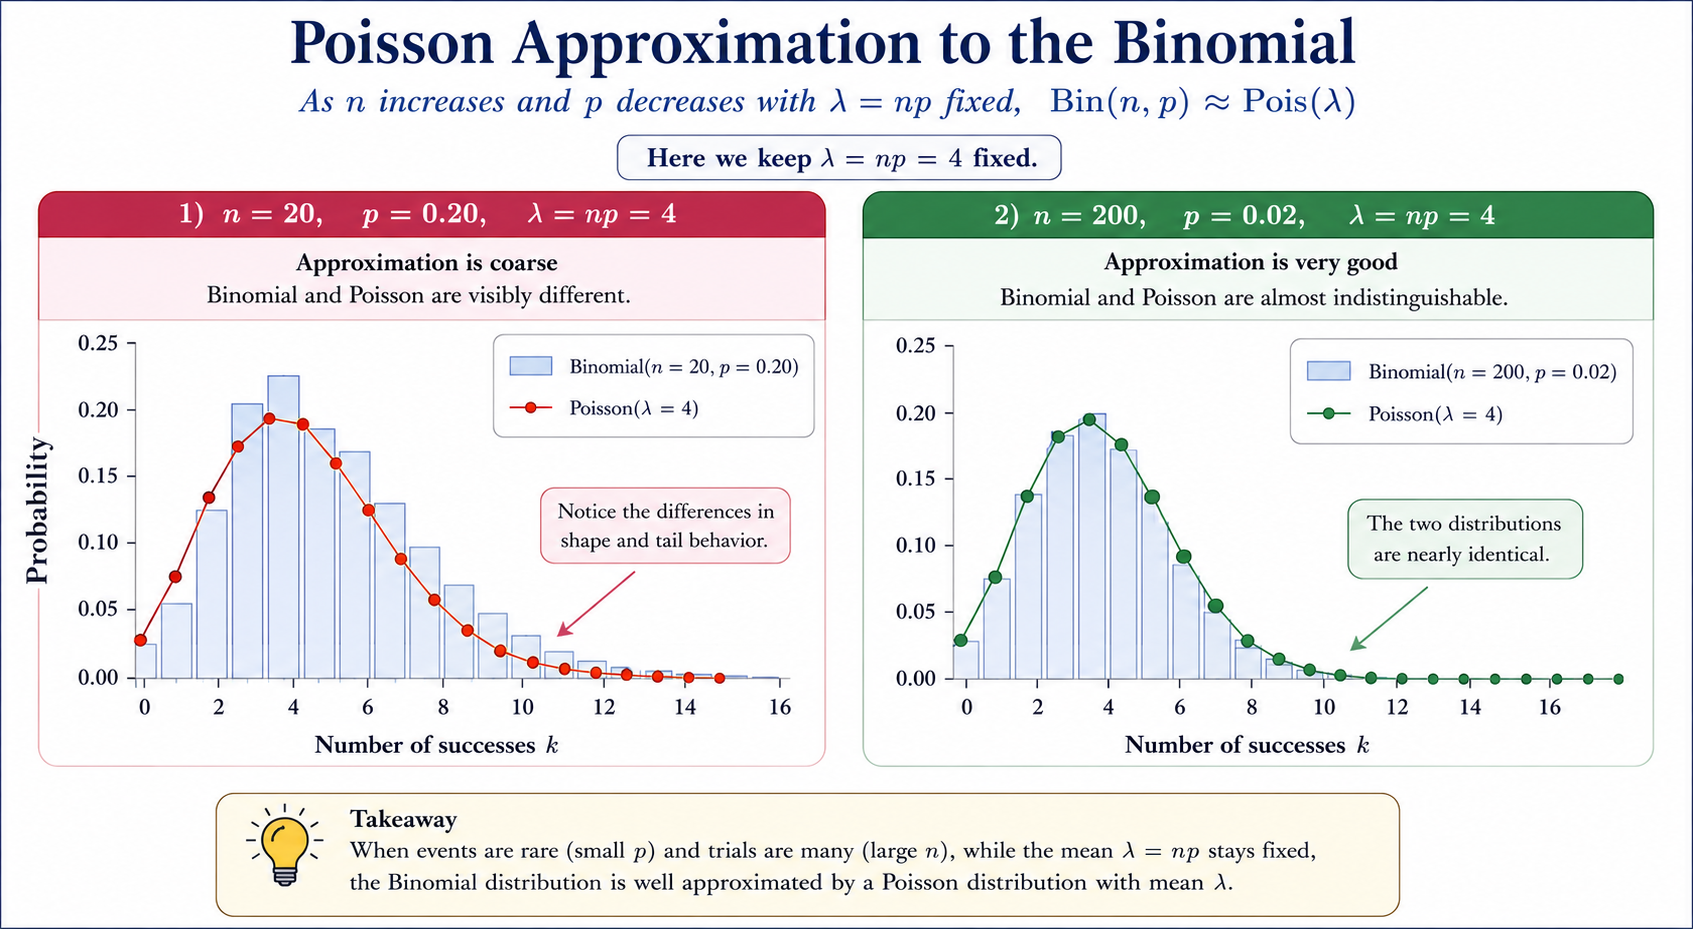
\includegraphics[
width=0.92\textwidth
]{assets/figures/pois.png}

\end{center}

\end{frame}












\begin{frame}{Example: Website Visitors}
Suppose $1{,}000{,}000$ people independently decide whether to visit a website.

Each visits with probability
\[
p=2\times 10^{-6}.
\]

Let
\[
X=\text{number of visitors}.
\]

Then
\[
X\sim \operatorname{Bin}(1{,}000{,}000,2\times 10^{-6}).
\]

Here
\[
\lambda=np=2.
\]

So
\[
X\approx \operatorname{Pois}(2).
\]

For example,
\[
\Prob(X=0)\approx e^{-2}.
\]

Note that it is computationally hard to compute $\mathbb{P}[X=k]$ directly from the Binomial PMF for different values of $k\in \mathbb{N}$:
\begin{equation}
    \mathbb{P}(X=k) = \frac{1000000!}{k! (1000000-k)!} (\frac{2}{10^6})^k(1-\frac{2}{10^6})^{1000000-k}
\end{equation}
\end{frame}



\begin{frame}{Summary}
\begin{itemize}
    \item Expectation is a probability-weighted average:
    \[
    \mathbb{E}(X)=\sum_x x\Prob(X=x).
    \]

    \item Linearity of Expectation:
    \[
    \mathbb{E}(X+Y)=\mathbb{E}(X)+\mathbb{E}(Y),
    \]
    with no independence required. Also works for linear combinations of finite number of random variabels.

    \item Fundamental bridge:
    \[
    \mathbb{E}(I_A)=\Prob(A).
    \]

    \item Variance measures spread:
\[
\begin{aligned}
\operatorname{Var}(X)
&\triangleq \mathbb{E}\!\left[(X-\mathbb{E}[X])^2\right]\\
&= \mathbb{E}[X^2]-(\mathbb{E}[X])^2
= \mathbb{E}[X^2]-\mu^2 \\[0.3em]
&= \mathbb{E}[X(X-1)] + \mathbb{E}[X] - (\mathbb{E}[X])^2
= \mathbb{E}[X(X-1)] + \mu - \mu^2.
\end{aligned}
\]
with no linearity property, except under zero correlation (independence).

    \item Poisson approximates Binomial when $n$ is large, $p$ is small, and $\lambda=np$ is moderate.
\end{itemize}


\begin{keybox}{Next lecture}
Continuous random variables.
\end{keybox}
\end{frame}